%!TEX TS-program = xelatex
\documentclass[a4paper,14pt]{article}
%%% Работа с русским языком
\usepackage[english,russian]{babel} %% загружает пакет многоязыковой вeрстки
\usepackage{fontspec} %% подготавливает загрузку шрифтов Open Type, True Type и др.
\defaultfontfeatures{Ligatures={TeX},Renderer=Basic} %% свойства шрифтов по умолчанию
\setmainfont[Ligatures={TeX,Historic}]{Times New Roman} %% задаeт основной шрифт документа
\setmonofont{Courier New} %% Моноширинный
\usepackage{indentfirst}
\frenchspacing

%%% Other packages
\usepackage{pdfpages}
\usepackage{fancyvrb}
\usepackage{fvextra}
\usepackage{icomma}
\usepackage{geometry}
\geometry{top=20mm}
\geometry{bottom=20mm}
\geometry{left=30mm}
\geometry{right=15mm}

\begin{document}
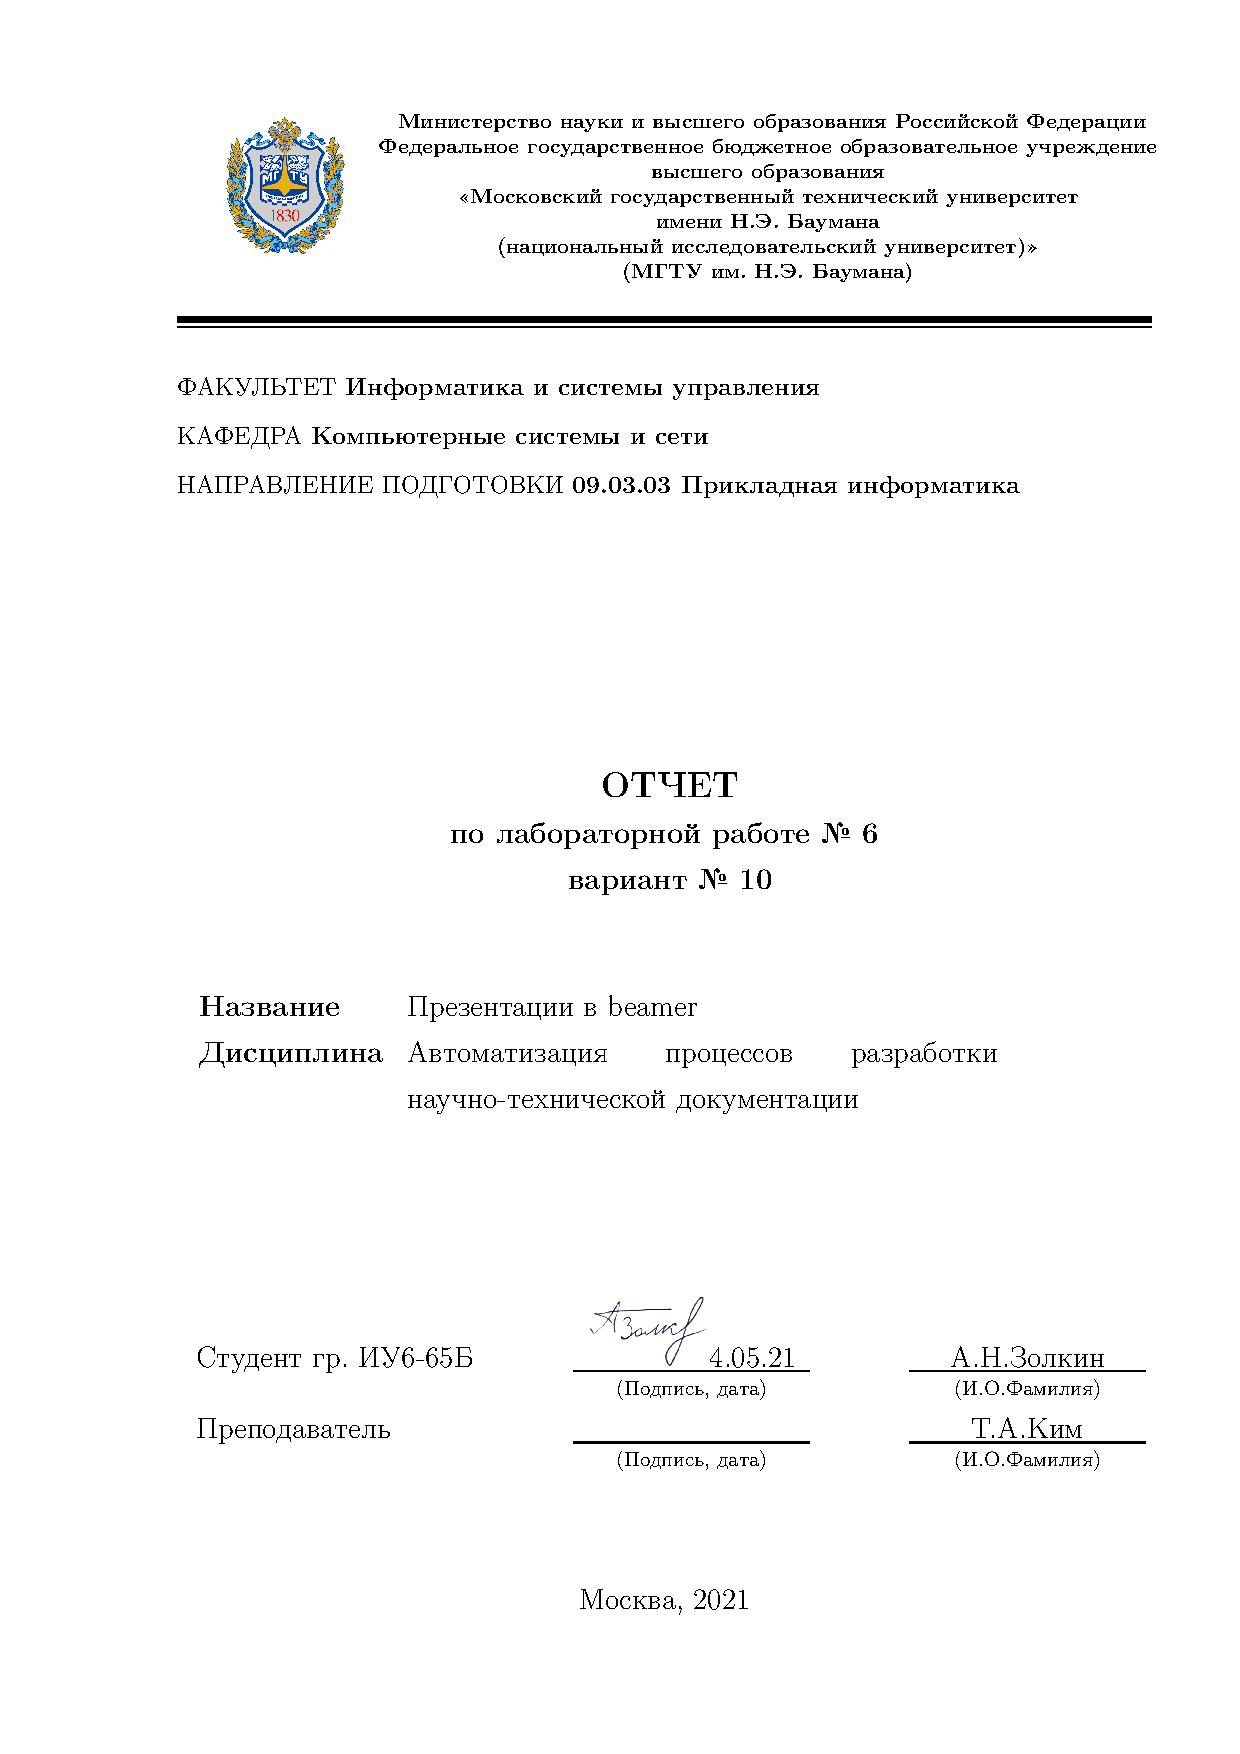
\includepdf[pages=-]{front-page.pdf}
\large{
    \par \textbf{Цель работы}: получить навыки по использованию \LaTeX как инструмента для создания строгих презентаций.

    \bigskip
    \texttt{\VerbatimInput[frame=lines, breaklines=true, breakanywhere=true]{lab6}}
    \bigskip

    
\includepdf[nup=1x3, delta=5mm 5mm, scale=0.9, frame, pages=-]{lab6.pdf}

    \large{
        \par \textbf{Вывод}: В ходе выполнения лабораторной работы были получены основные навыки использования \LaTeX для создания презентаций.
    }
}
\end{document}
